\documentclass[14pt]{extarticle}

\usepackage[T2A]{fontenc}
\usepackage[utf8]{inputenc}
\usepackage[russian]{babel}
\usepackage{hyphenat}

\usepackage{mathptmx}
\usepackage{gensymb}
\usepackage[left = \flqq{},right = \frqq{}]{dirtytalk}

\usepackage{amsmath}

\usepackage{geometry}
\geometry{
	a4paper,
	top=20mm,
	bottom=23mm,
	footskip=10mm,
	left=25mm,
	right=15mm
}
\setlength{\parindent}{10mm}
\renewcommand{\baselinestretch}{1.5}

\usepackage{fancyhdr}
\pagestyle{fancy}
\renewcommand{\headrulewidth}{0pt}
\lhead{}
\chead{}
\rhead{}
\lfoot{}
\cfoot{}
\rfoot{\thepage}

\usepackage{indentfirst}

\usepackage{enumitem}

\usepackage{graphicx}
\usepackage[labelformat=simple]{subcaption}
\renewcommand{\thesubfigure}{\textit{\asbuk{subfigure})}}
\usepackage{setspace}
\usepackage[font=small, labelsep=period]{caption}
\captionsetup[figure]{font={small,stretch=1.0}}

\usepackage{titlesec}
\titleformat{\section}[hang]{\large\bf}{\thesection.}{.5em}{}{}
\titleformat{\subsection}[hang]{\normalsize\bf}{\thesubsection.}{.5em}{}{}
\titleformat{\subsubsection}[hang]{\normalsize\bf}{\thesubsubsection.}{.5em}{}{}
\titlespacing*{\section}{0mm}{6pt}{6pt}
\titlespacing*{\subsection}{0mm}{6pt}{6pt}
\titlespacing*{\subsubsection}{0mm}{6pt}{6pt}

\usepackage{titletoc}
\titlecontents{section}[3mm]{}{\thecontentslabel.\space\filright}{}{\titlerule*[1pc]{.}\contentspage}
\titlecontents{subsection}[6mm]{}{\thecontentslabel.\space\filright}{}{\titlerule*[1pc]{.}\contentspage}
\titlecontents{subsubsection}[9mm]{}{\thecontentslabel.\space\filright}{}{\titlerule*[1pc]{.}\contentspage}

\usepackage{enumitem}
\setlist{nosep}

\begin{document}
	\setlength{\abovedisplayskip}{6pt}
	\setlength{\belowdisplayskip}{6pt}
	\setlength{\belowcaptionskip}{-15pt}
	\pagenumbering{arabic}
	\setcounter{page}{3}
	\thispagestyle{fancy}
\tableofcontents
\newpage
\section{Введение}
В Институте ядерной физики им. Г. И. Будкера СО РАН проводятся эксперименты на электрон-позитронном коллайдере ВЭПП-2000. Коллайдер имеет два места встречи пучков, в которых установлены детекторы КМД-3 (криогенный магнитный детектор) и СНД (сферический нейтральный детектор). В программу проекта ВЭПП-2000 включено измерение сечений процессов, наблюдаемых при столкновениях электронов и позитронов в диапазоне энергий до 2 ГэВ \cite{shatunov}. В число изучаемых процессов входят процессы с фотонами в конечном состоянии.

Для регистрации фотонов в детекторе КМД-3 используется жидкоксеноновый (LXe) калориметр. Фотон, попадая в калориметр, порождает электромагнитный ливень из вторичных электронов, позитронов и фотонов. Частицы ливня регистрируются сигнальными полосками, расположенными на слоях калориметра. Сработавшие сигнальные полоски группируются в кластеры.

При столкновениях электронов $e^-$ и позитронов $e^+$ большое сечение рождения имеют процессы, содержащие нейтральный пион $\pi^0$ в конечном состоянии. Одним из таких процессов является $e^- e^+ \rightarrow \pi^0 \gamma$. Нейтральный пион с вероятностью 99\% распадается на два фотона $\gamma$. Минимальный угол между фотонами при более высокой энергии пи-мезона становится меньше, и при значении $E_{\pi^0}$ = 1 ГэВ этот угол составляет 0,27 радиана. Электромагнитные ливни таких фотонов в калориметре могут перекрываться, и появляется вероятность принять два слившихся кластера, образованных двумя фотонами, за одиночный кластер от одного фотона. Чтобы увеличить статистику событий, повысить точность измерения сечения и других параметров процесса, необходимо разделять такие кластеры.

Таким образом, требуется разработать алгоритм различения однофотонных и двухфотонных кластеров в LXe калориметре детектора КМД-3. Для решения этой задачи выполнены следующие шаги:
\begin{itemize}
	\item описание детектора КМД-3 и LXe калориметра,
	\item подготовка данных для обработки,
	\item обзор библиотеки TMVA 4 и метода BDT,
	\item анализ задачи разделения кластеров,
	\item реализация алгоритма разделения кластеров с помощью метода BDT.
\end{itemize}

Результаты данной работы планируется сравнить с результатами, полученными в работах \cite{lakomov,rabusov}.
\section{Детектор КМД-3 и LXe калориметр}
На рис.~\ref{fig:cmd3} представлена схема криогенного магнитного детектора КМД-3.
\begin{figure}[h!]
	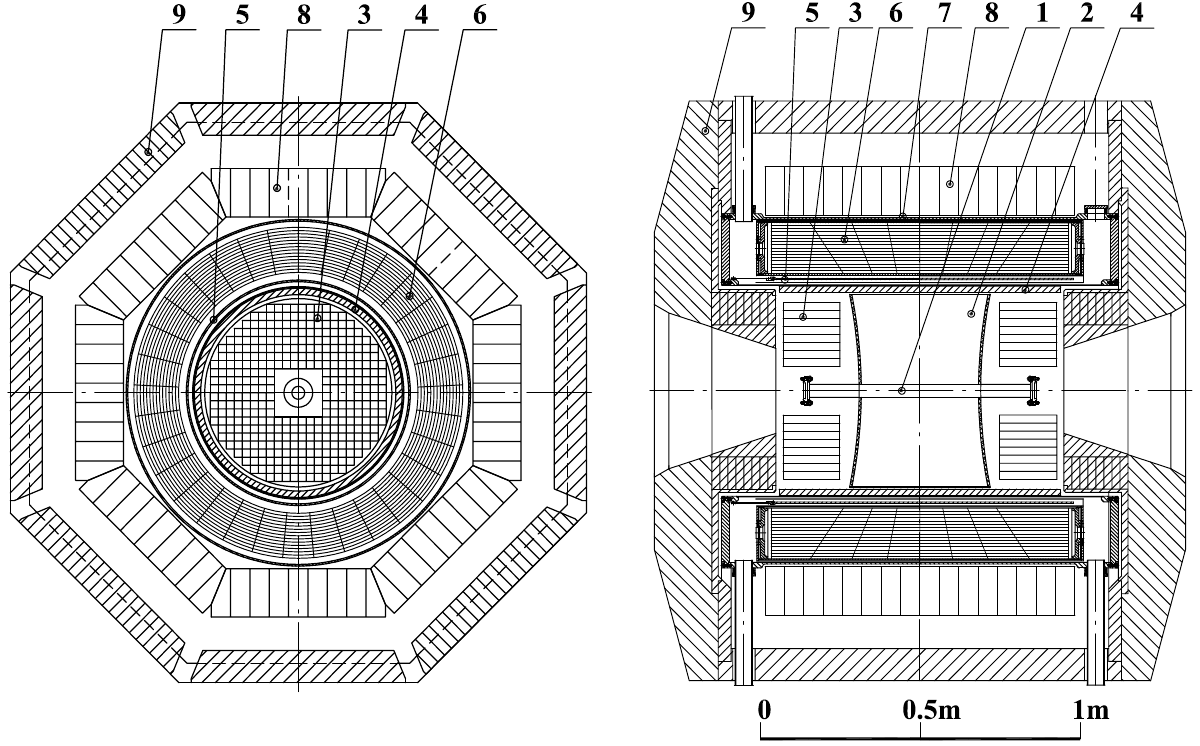
\includegraphics[width=\linewidth]{../pics/cmd3-2.png}
	\caption{Схема детектора КМД-3: 1 -- вакуумная камера, 2 - дрейфовая камера, 3 -- торцевой BGO калориметр, 4 -- Z-камера, 5 -- сверхпроводящий соленоид, 6 -- цилиндрический жидкоксеноновый калориметр, 7 -- времяпролётная система, 8 -- цилиндрический CsI калориметр, 9 -- ярмо магнита \cite{shebalin}}
	\label{fig:cmd3}
\end{figure}

Цилиндрический электромагнитный калориметр детектора регистрирует фотоны и электроны, которые вылетают под большими углами к оси пучков (от $39\degree$ до $141\degree$), и охватывает телесный угол $0,8 \cdot 4\pi$. Он состоит из двух соосных подсистем: жидкоксенонового LXe калориметра и кристаллического CsI калориметра.

Жидкоксеноновый калориметр образован семью соосными катодами и восемью анодами, образующими систему ионизационных камер. Структура электродов LXe калориметра представлена на рис.~\ref{fig:lxe-electrodes} \cite{shebalin}.

\begin{figure}[h!]
	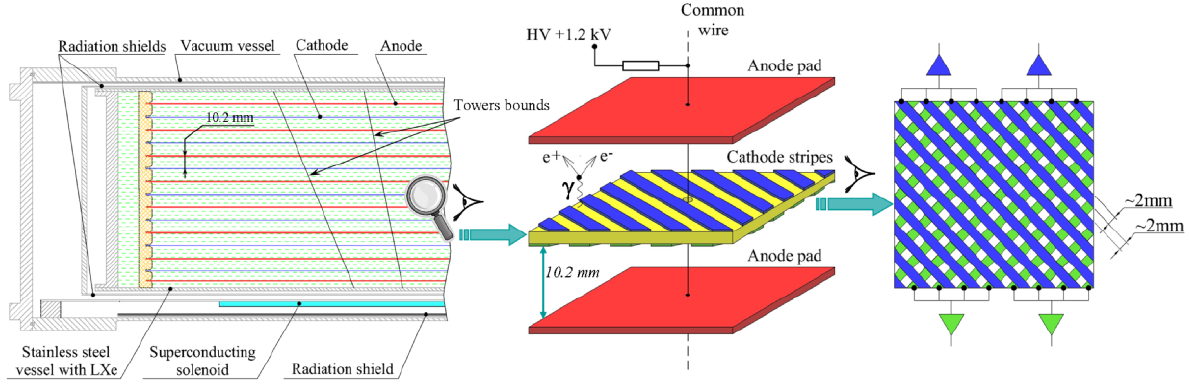
\includegraphics[width=\linewidth]{../pics/lxe-electrodes.png}
	\caption{Структура электродов жидкоксенонового калориметра}
	\label{fig:lxe-electrodes}
\end{figure}

Поверхность каждого анода разделена на 264 прямоугольные площадки -- восемь вдоль оси пучков $Z$, тридцать три в перпендикулярной ей плоскости $R,\varphi$. Площадки с одинаковым положением по $Z$ и $\varphi$ соединены проводником в \say{башню}. Такая \say{башня} ориентирована в место встречи пучков. Аноды используются для измерения выделенной энергии.

Каждый катод разбит на 2112 полосок. Полоски объединены в группы по четыре, и с каждой такой группы сигнал снимается по одному каналу. На противоположных сторонах катода полоски ориентированы взаимно перпендикулярно и находятся под углом $45\degree$ к оси пучков $Z$ \cite{shebalin}. Такая структура катода используется для восстановления координат кластера.

Регистрация фотонов производится путём сбора информации о частицах электромагнитного ливня, порождённого при взаимодействии фотона с материалом калориметра. LXe калориметр позволяет измерять координаты с погрешностью от 0,7 мм для первого слоя до 1,4 мм для шестого слоя \cite{Epifanov_2011,lxe_2009}. Точность измерения энергии составляет примерно 8,5\% для нейтральных пи-мезонов \cite{Anisenkov_2014}.
\section{Формат входных данных с калориметра}
\section{Библиотека TMVA и метод BDT}
Библиотека TMVA (The Toolkit for Multivariate Analysis) предоставляет среду для параллельного вычисления и применения методов многомерной классификации и, начиная с версии TMVA 4, многомерной регрессии. В данной библиотеке представлены только алгоритмы машинного обучения с учителем. Они используют тренировочные события с известным результатом, чтобы определить отображение, которое описывает либо критерии классификации, либо регрессионное приближение для функции результата. Среда TMVA разработана в основном для нужд физики высоких энергий, но может применяться и в других областях \cite{tmva4}.

В данной работе используется метод BDT (boosted decision trees), основанный на нахождении множества деревьев решений с присвоенными им весами. Дерево решений -- это классификатор, построенный в виде двоичного дерева. Пример такого дерева изображён на рис.~\ref{fig:dectree}.

\begin{figure}[h!]
	\centering
	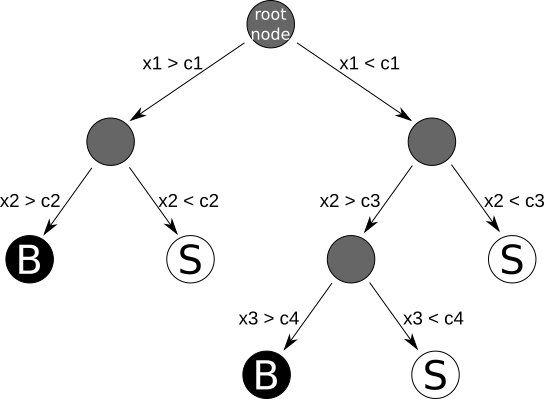
\includegraphics[width=0.7\linewidth]{../pics/decision.png}
	\caption{Пример дерева решений. Решения принимаются на основе переменных $x1$, $x2$, $x3$, критериями являются величины $c1$, $c2$, $c3$, $c4$.}
	\label{fig:dectree}
\end{figure}

Задача алгоритма, использующего дерево решений, заключается в том, чтобы пройти это дерево, начиная с корневого узла, и закончить на одном из листьев дерева. В каждом узле находится критерий выбора дочернего узла по значению одной из переменных. В результате алгоритм относит событие к категории сигнальных или фоновых.

Тренировка дерева производится поэтапно, начиная с корневого узла. Выбирается критерий, наиболее эффективно делящий события на фоновые и сигнальные, то есть дающий наибольшую долю правильно классифицированных событий в обеих категориях. Такая же процедура выбора критерия выполняется на каждом из двух образовавшихся подмножеств событий и так далее до определённой глубины дерева. Таким образом, фазовое пространство оказывается поделено на сегменты, помеченные как сигнал или фон в зависимости от того, событий какого типа больше всего попало в данный сегмент при тренировке алгоритма.

Достоинства дерева решений -- простота описания и интерпретации, а также возможность разбивать фазовое пространство на большое число гиперкубов, обозначаемых как фон или сигнал -- в отличие от анализа на основе совокупности пороговых значений, которая выделяет лишь один гиперкуб. Недостатком дерева решений является его чувствительность к статистическим флуктуациям в тренировочном наборе событий. Например, две переменные, одинаково влияющие на классификацию событий, под действием флуктуаций могут идти в разном порядке следования сравнений, что изменит и всю дальнейшую структуру дерева, в итоге воздействуя на результат классификации.

Для уменьшения флуктуаций, метод BDT использует бустинг деревьев. Для этого данные делятся на некоторое количество ансамблей $N$, и на каждом ансамбле тренируется по одному дереву решений. В итоге получается $N$ деревьев, каждое из которых имеет свой уровень разделения и даёт свой отклик на одно и то же событие. Деревьям присваиваются веса в зависимости от качества разделения. Итоговая величина $r$ отклика на событие вычисляется как средневзвешенное по всем деревьям:
\begin{align*}
r = \sum_i \omega_i r_i,
\end{align*}
где $\omega_i$ -- вес $i$-го дерева, $r_i$ -- отклик $i$-го дерева \cite{tmva4}.
\section{Алгоритм разделения кластеров}
Задача алгоритма -- имея координаты совокупности точек и связанные с ними значения энергии, классифицировать событие как сигнальное или фоновое. Сигнальным событием считается появление кластера, сгенерированного только одним фотоном, а фоновое событие -- это регистрация слившихся кластеров.

Для решения этой задачи в среде C++/ROOT с использованием библиотеки TMVA 4 разработаны следующие процедуры:
\begin{enumerate}
	\item генерация набора данных для обучения и проверки алгоритма,
	\item реализация алгоритма при помощи метода BDT,
	\item проверка работы алгоритма на некотором наборе данных.
\end{enumerate}


\section{Результаты}
\section{Заключение}


\bibliographystyle{unsrt}
\addcontentsline{toc}{section}{Список литературы}
\bibliography{coursework}
\end{document}